\documentclass[12pt, a4paper]{article}

\usepackage{import}
\usepackage{standalone}

\usepackage[top=4cm, right=2cm, bottom=2.7cm, left=2cm]{geometry}

\usepackage{wrapfig}
\usepackage{tabulary}
\usepackage{float}
\usepackage{pifont}
\usepackage{background}
\usepackage{tikz}


\pagestyle{empty}
\setlength{\parindent}{0pt}

\begin{document}
	\begin{minipage}{\textwidth}
		\section{Robotselectie \hfill\small Bron: Bebras}
			
			Meneer Bever bezit 15 robots die hieronder zijn afgebeeld. Deze robots kunnen naar opdrachten luisteren en ze uitvoeren.
			
			%image
			\begin{figure}[H]
				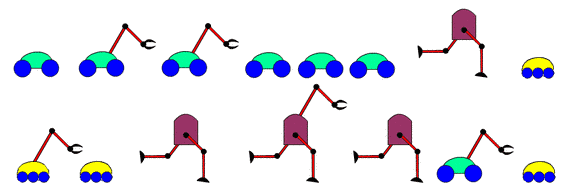
\includegraphics[width=\linewidth]{image1}
			\end{figure}
			
			Meneer Bever wil de robots naar de beverdam sturen die hij nodig heeft om hem te helpen bij zijn reparaties. Daarom geeft hij de volgende opdrachten aan alle robots:
			
			\begin{enumerate}
				\item Als je drie kleine wieltjes hebt, stop dan met het volgen van deze bevelen!
				\item Heb je zowel twee benen en een arm, ga dan onmiddellijk naar de beverdam!
				\item Heb je twee benen of een arm, stop dan met het volgen van deze bevelen!
				\item Ga naar de beverdam!
			\end{enumerate}
			
			Hoeveel robots zullen er uiteindelijk aankomen bij de beverdam nadat meneer Bever deze reeks opdrachten heeft gegeven?
			
			%\begin{center}
			%	Antwoord: \raisebox{-0.2cm}{\rule{5cm}{0.4pt}}
			%\end{center}


	\end{minipage} \\ \\ 
		
\end{document}